\begin{figure}[htbp]
\centering
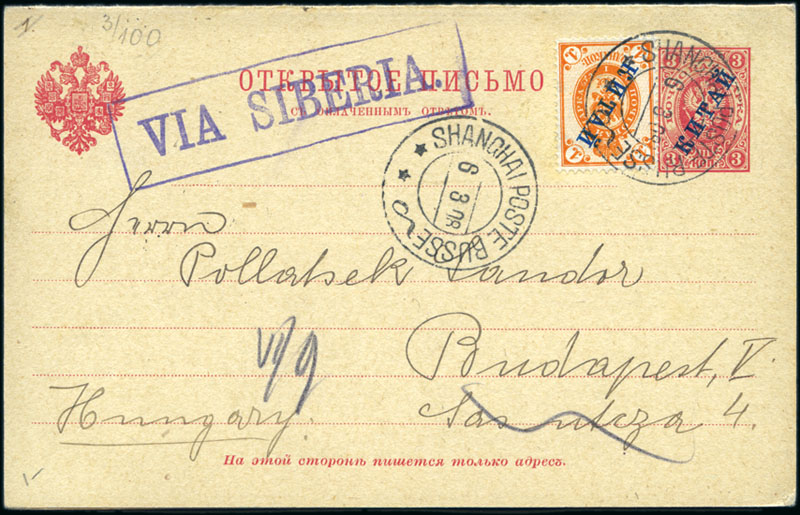
\includegraphics[width=.95\textwidth]{../russian-post-offices-in-china/10071.jpg}
\caption{
10071	SHANGHAI: 1908 "KITAI" 3k (+3k) reply paid letter card to Budapest 
with "via Siberia" hs, uprated with "KITAI" 1k both cancelled by Shanghai 
6.3.08 cds (T\&S type 6B), Budapest bs, with unused half pre-cancelled simultaneously.
\euro150.00. 
}  
\end{figure}

Lorem ipsum dolor sit amet, consectetur adipiscing elit. Sed nibh justo, dictum sed cursus ac, lobortis et lacus. Vestibulum vitae justo enim. Quisque laoreet elementum felis, ut sodales arcu viverra a. Sed molestie odio vulputate sem rutrum a sagittis est rutrum. Morbi dapibus hendrerit magna, sit amet commodo massa posuere sit amet. Duis pharetra quam scelerisque est lobortis fringilla. Maecenas venenatis feugiat lectus, vel facilisis odio pharetra quis. Etiam at nisl eros, sit amet suscipit lorem. Lorem ipsum dolor sit amet, consectetur adipiscing elit. Sed augue nunc, ornare eget congue sit amet, laoreet vel augue. Morbi vel justo quis ipsum adipiscing egestas vitae non est. Vivamus ac quam quam. Nullam pharetra
                                                    interdum mauris, rutrum pulvinar ligula condimentum id. Donec et blandit lorem. 

\begin{figure}[htbp]
\centering
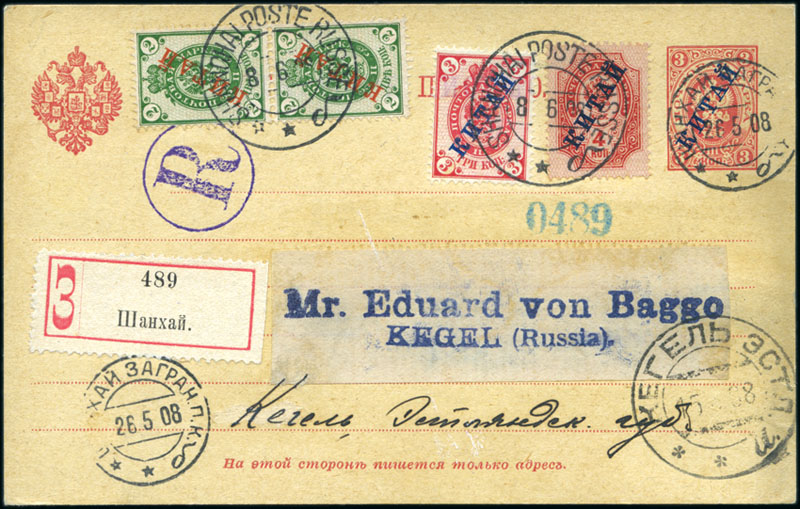
\includegraphics[width=.95\textwidth]{../russian-post-offices-in-china/10072.jpg}
\caption{
10072	SHANGHAI: 1908 "KITAI" 3k postcard registered to Kegel 
(in modern day Estonia), uprated with "KITAI" 2k (2), 3k and 4k, 
unusually paying the 4k foreign postcard rate and 10k reg'n fee 
(possibly because the address is in English), with imprint cancelled 
by Shanghai 25.5.08 cds (T\&S type 5B, Julian calendar) and stamps tied 
by Shanghai 8.6.08 cds (T\&S type 6B, Gregorian calendar), with registered
label in Cyrillic and encircled 'R' normally applied to foreign-bound 
registered mail, Kegel arrival, attractive franking.
\euro400.00 
}  
\end{figure}

Lorem ipsum dolor sit amet, consectetur adipiscing elit. Sed nibh justo, dictum sed cursus ac, lobortis et lacus. Vestibulum vitae justo enim. Quisque laoreet elementum felis, ut sodales arcu viverra a. Sed molestie odio vulputate sem rutrum a sagittis est rutrum. Morbi dapibus hendrerit magna, sit amet commodo massa posuere sit amet. Duis pharetra quam scelerisque est lobortis fringilla. Maecenas venenatis feugiat lectus, vel facilisis odio pharetra quis. Etiam at nisl eros, sit amet suscipit lorem. Lorem ipsum dolor sit amet, consectetur adipiscing elit. Sed augue nunc, ornare eget congue sit amet, laoreet vel augue. Morbi vel justo quis ipsum adipiscing egestas vitae non est. Vivamus ac quam quam. Nullam pharetra
                                                    interdum mauris, rutrum pulvinar ligula condimentum id. Donec et blandit lorem. 

\begin{figure}[htbp]
\centering
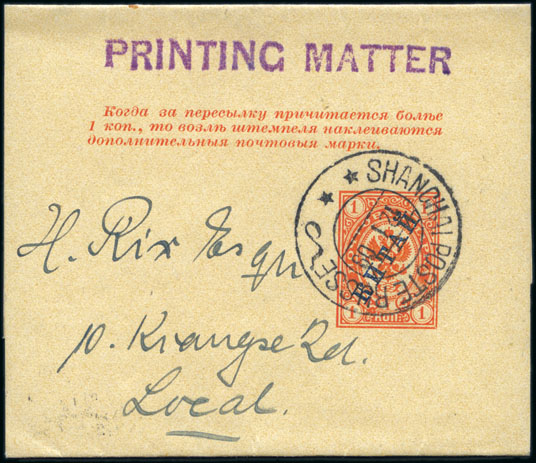
\includegraphics[width=.95\textwidth]{../russian-post-offices-in-china/10073.jpg}
\caption{
10073	SHANGHAI: 1909 "KITAI" 1k newspaper wrapper sent locally in Shanghai, 
cancelled by Shanghai 21.1.09 cds (T\&S type 6B), very fine and scarce 
printed matter rate usage.
\euro 200.00 
}  
\end{figure}

\begin{figure}[htbp]
\centering
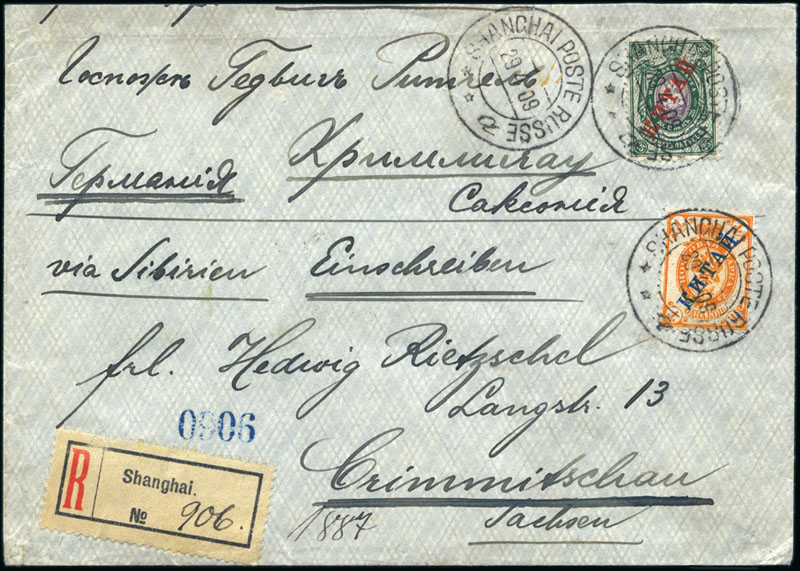
\includegraphics[width=.95\textwidth]{../russian-post-offices-in-china/10074.jpg}
\caption{
10074	SHANGHAI: 1909 Cover sent registered to Germany with "KITAI" 1k and 
25k tied by Shanghai 29.4.09 cds (T\&S type 6A) with unusual black and red 
registered label in English adjacent and reg'n number repeated by blue 
hs, fine and scarce use of the 25k
\euro 300.00
}  
\end{figure}

\begin{figure}[htbp]
\centering
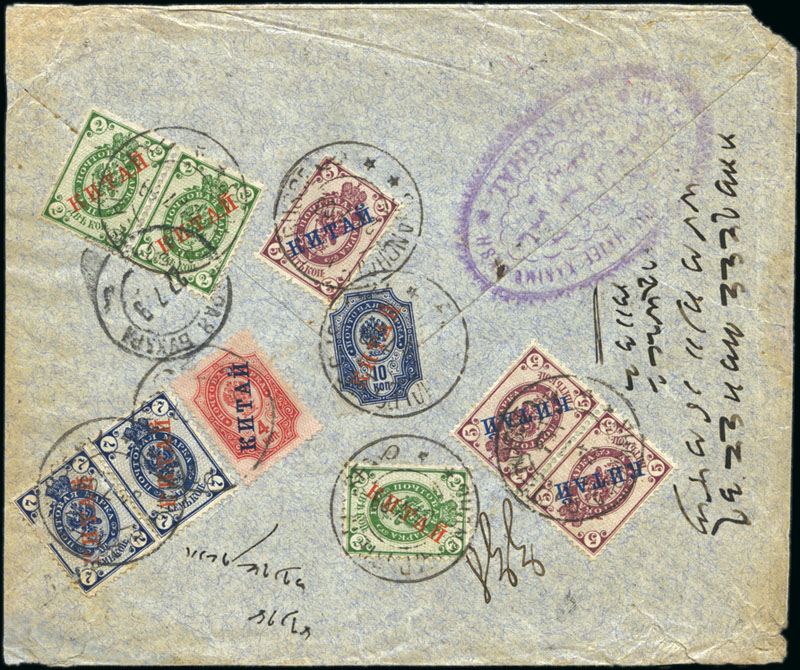
\includegraphics[width=.95\textwidth]{../russian-post-offices-in-china/10075.jpg}
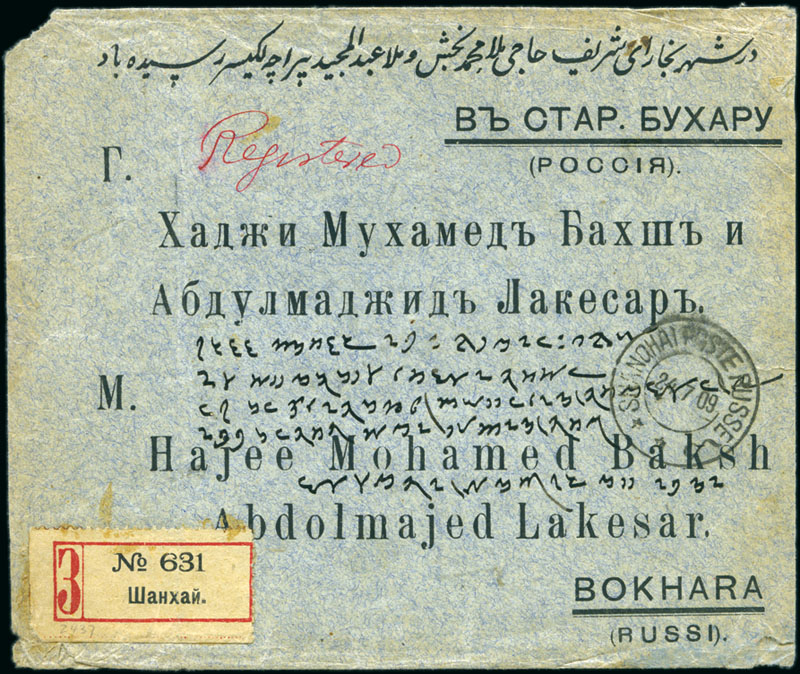
\includegraphics[width=.95\textwidth]{../russian-post-offices-in-china/10075-1.jpg}
\caption{
10075		ZoomSHANGHAI: 1909 Cover addressed in Farsi, Russian and English 
registered to Bukhara (in modern day Uzbekistan), with "KITAI" 2k (3), 4k, 
5k (3) and 7k (2) and 10k, paying six times the 7k internal rate plus reg'n 
fee, all tied by Shanghai 24.7.09 cds (T\&S type 6B, Gregorian calendar), 
obverse with reg'n label in Cyrillic, small cover corner fault, a scarce 
rate and attractive multiple franking.

Note: Type 6 cancels were only intended for use on mail to foreign countries.
\euro 300.00 
}  
\end{figure}
          